\chapter{Uso de refugios}
Para varias especies los refugios son fundamentales para la protección de predadores y  condiciones climaticas (especialmente para animales de sangre fría, como las tortugas). En especies relativamente solitarias, los individuos pasan un tiempo considerable solos en los refugios y tienen pocos encuentros directos fuera de la epoca de apareamiento.
Ejemplos de estas especies incluyen a los mapaches, zorros rojos, orangutanes y algunas especies de abejas, avispas y murcielagos. Para estas poblaciones de animales salvajes, monitorear y entender estos refugios puede ayudar a establecer patrones sociales de los individuos. 

En distintos campos cercanos a la zona de medición (San Antonio Oeste, provincia de Río Negro) estan introduciendo ganado al habitad de las tortugas, es importante entender si presenta una amenaza para la integridad de los refugios y entender el patron de movimiento  de las tortugas sobre los mismos, junto con las caracteristicas geograficas de los refugios mas usados.

\section{Refugios en el mapa}
Para determinar el refugio donde paso la noche la tortuga se tomaron dos criterios, uno para cada una de las metodologias de medicion en los sets de datos. Para el tortugometro se tomo el ultimo punto tomado de la tortuga en un día de medición y se pidió la condicion de que haya sido tomado despues de las 20 horas, en base a las anotaciones tomadas por el grupo, las tortugas generalmente  se encontraban en el refugio cuando quitaban los tortugometros despues de este horario. A este punto nuevo se le asigna un label de refugio y un enlace con la tortuga que paso la noche en ese refugio. A medida que se añade otro refugio primero se verifica que presente una distancia mayor a 20 metros con todos los otros refugios labeleados, en caso que la distancia es menor a 20 metros a por ejemplo el refugio 1, se dice que la tortuga estuvo en el refugio 1. 

Para los datos tomados por los i-gotU, se decidió mirar primero las distancias entre el ultimo punto medido (21 horas) de algún día monitoreado con el primer punto del día siguiente (6 horas). Y tambien se miraron las distancias entre el primer punto de algun dia de monitoreo con el segundo punto (6 horas y 6:15 respectivamente). En la Fig. \ref{fig:distancias} se muestran los histogramas de las distancias entre los puntos. Se observa que entre el ultimo punto de la noche y el primero de la mañana distancias mayores a 20 metros son muy probables con varias mediciónes de distancias del orden de los 50 o 100 metros, lo que nos diría que la tortuga todavía no se encuentra en el refugio a esa hora (21 horas). En cambio, entre el primer punto del día y el segundo punto, las distancias menores a 20 metros son las mas probables, lo que nos diría que la tortuga todavía no abandonó el refugio entre las 6 y las 6:15. Por eso para los datos de los i-gotU se decidió tomar el primer punto del día como la posición del refugio y se siguió el mismo procedimiento que para los datos del tortugometro. De cara a las proximas campañas se decidió mantener las mediciónes del i-gotU entre las 21 y las 6 horas, pero disminuyendo la frecuencia de muestreo. 


\begin{figure}[ht]
    \begin{center}
        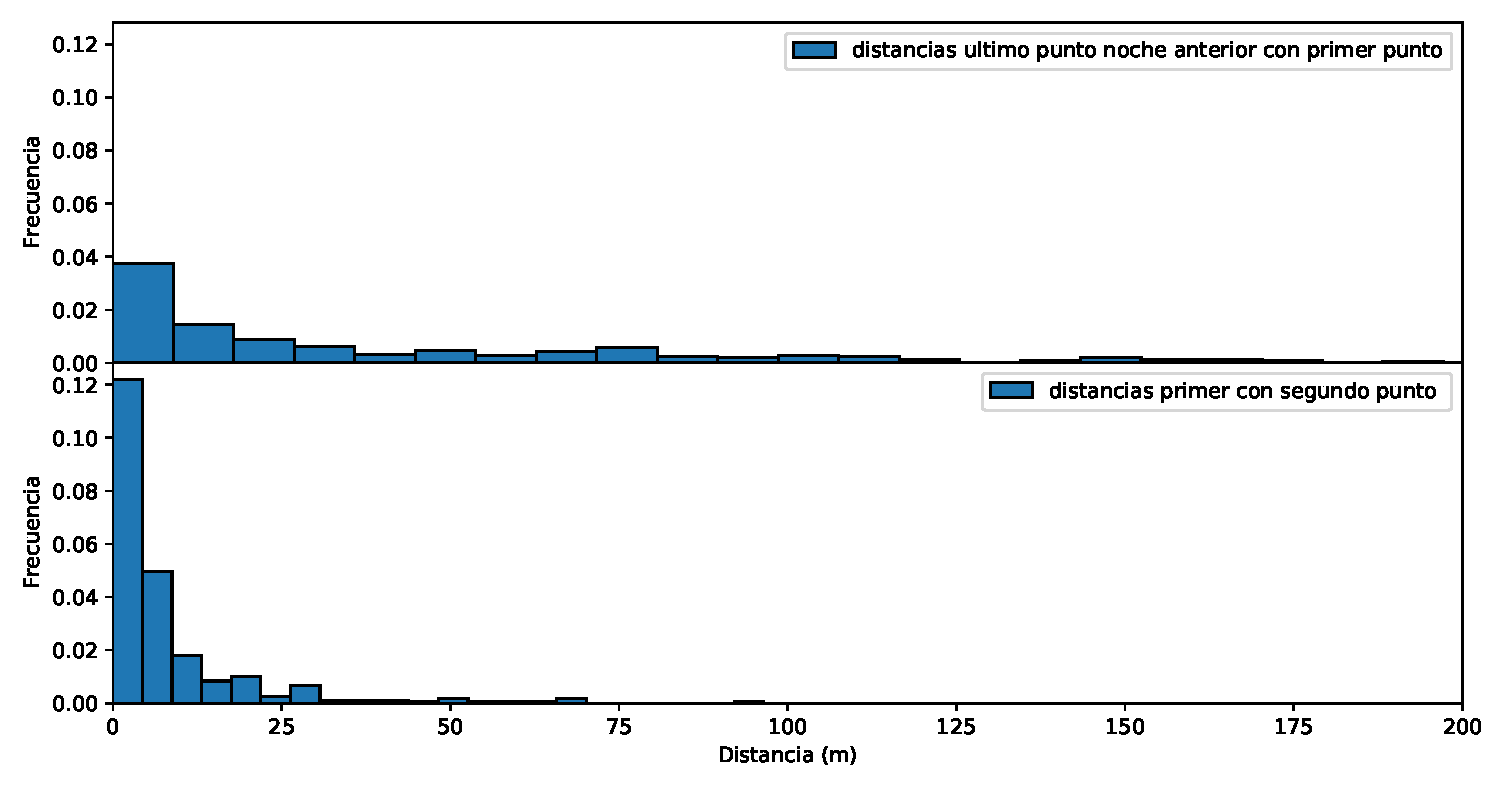
\includegraphics[width=1.4\imsize]{Chap3/Distancias_primer_ult_con_deteterminar_criterio_ref.pdf}
        \caption[Histogramas de las distancias entre los puntos de los datos de i-gotU.]{ Histogramas de las distancias entre los puntos de los datos de i-gotU. Arriba se muestra la distancia entre el ultimo punto del dia anterior y el primer punto del dia siguiente. Abajo se muestra la distancia entre el primer punto del dia y el segundo punto del dia.} 
        \label{fig:distancias}
        \end{center}
\end{figure} 

Se graficaron los refugios encontrados en un mapa utilizando la librería Folium, los mapas fueron guardados en formato html para el facil acceso a los mismos, al clickear en un refugio sobre el html aparece un cartel con las tortugas que pasaron la noche en el refugio. En las Fig. \ref{fig:refus_campanas_con_labels} y \ref{fig:refus_igotu_labels} se muestran los mapas de los refugios encontrados para los datos de las campañas y los datos de i-gotU respectivamente.


\begin{figure}[ht]
    \begin{center}
        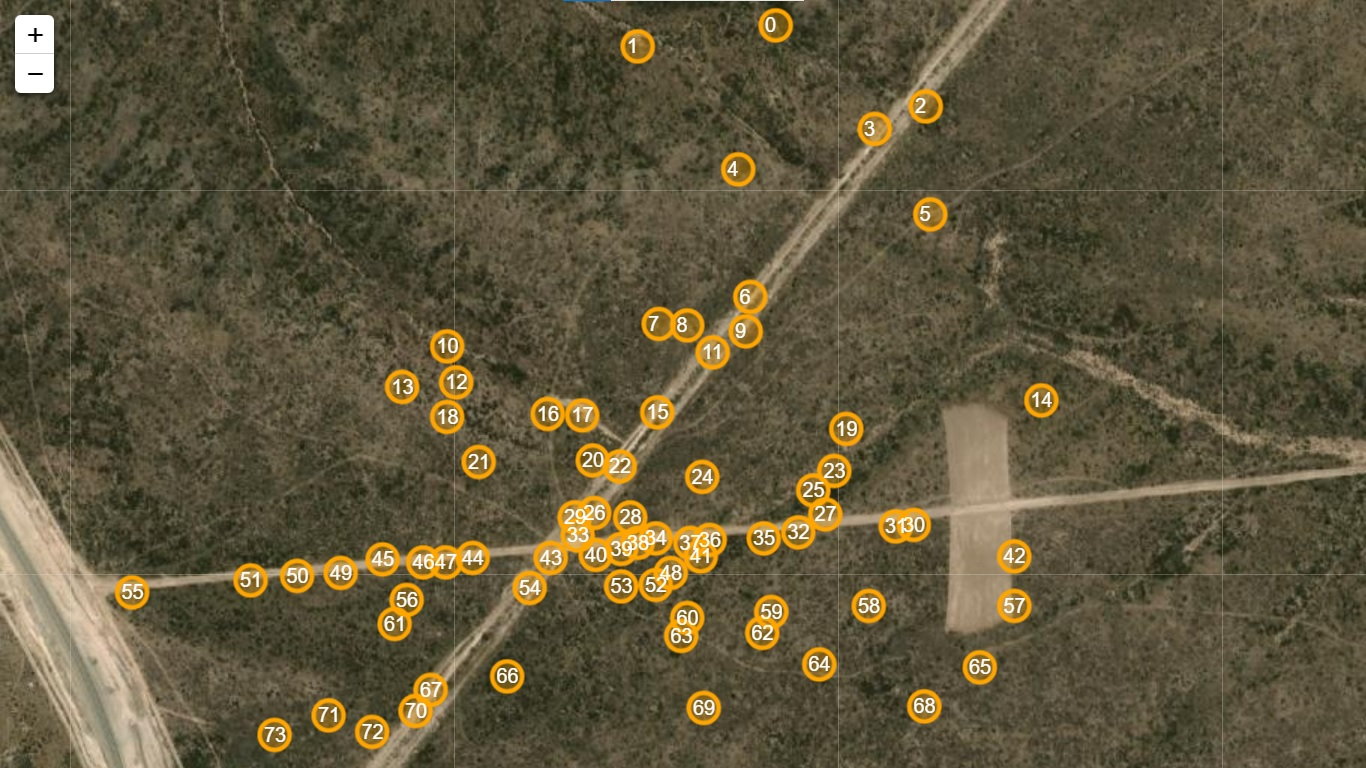
\includegraphics[width=\imsize]{Chap3/map_refugies_with_labels.jpg}
        \caption{Distribución geográfica de los refugios encontrados para los datos provenientes de las campañas.} 
        \label{fig:refus_campanas_con_labels}
        
        \end{center}
\end{figure} 

\begin{figure}[ht]
    \begin{center}
        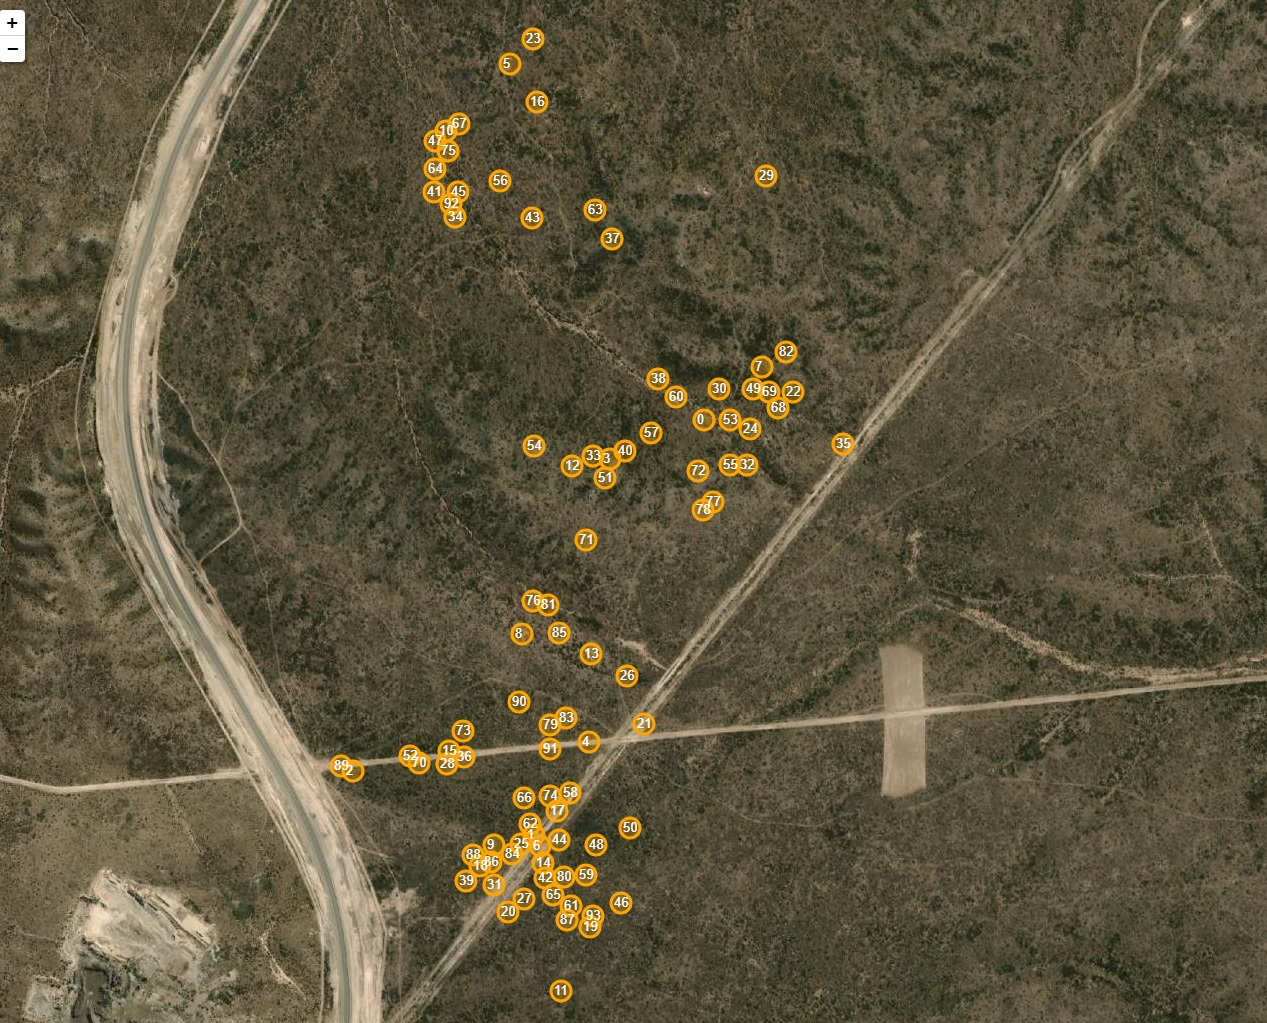
\includegraphics[width=\imsize]{Chap3/map_refugies_with_labels_IGOTo.jpg}
        \caption{Distribución geográfica de los refugios encontrados para los datos provenientes de los datos de i-gotU.} 
        \label{fig:refus_igotu_labels}
        
        \end{center}
\end{figure} 

En base a observaciónes de directas de campo \cite{Erika} se espera que las tortugas machos tengan una distribución de refugios mas amplia en el espacio que las hembras.  Para verificar esta hipotesis se definieron dos metricas, centro de masa de refugios y distancia media entre refugios. El centro de masa se define como:
\begin{center}
    

$$X_{centro}= \sum^{N -1}_{n=0} \frac{i_{n} X_n}{I_{totales}}.$$
\end{center}
Donde $I_{totales}$ es la cantidad de noches donde se registro que la tortuga durmio en un refugio (depende de cada tortuga), $X_n$ es la coordenada X del refugio n, $i_{n}$ es la cantidad de noches que la tortuga durmio en el refugio n y N la cantidad de refugios totales.  Este proceso se calcula para todas las tortugas. 
Partiendo de $X_{centro}$, la distancia media  espacial de los refugios se calcula como:
$$D = \sum^{N -1}_{n=0} \frac{|X_n i_n - X_{centro}|}{I_{totales}}.$$
\label{eq:distancia_media_refugios}
Esta metrica fue calculada para todas las tortugas y  promediada para  machos y hembras. Se encontro para los machos $\overline{D}_m =  (128\pm66)\,\text{m}$ y para las hembras     $\overline{D}_h = (122\pm82)\,\text{m}$. Es decir que no se encontraron diferencias significativas en la distribucion espacial de refugios  entre machos y hembras.
\section{Redes bipartitas de refugios}
Se armaron redes bipartitas con nodos refugios y nodos tortugas. Los nodos refugios solo estan conectados con nodos tortugas.  Partiendo de todos los labels de refugios con las tortugas que pasaron noche en ese refugio se armaron las redes bipartias para los datos tomados por los tortugometros y los datos tomados con los i-gotU, figuras respectivamente.%chequear


\begin{itemize}
    \item Criterio para identificar refugio, redes bipartitas de refus
    \item Distribucion espacial de los refugios con la definicion que use
    \item Paths de refugios y acumulada de noches en refugios (material adicional gif de refugies paths)
    \item proyeccion en solo refugios, mapa con proyeccion y metricas asociadas 
    \item Mantel test entre matriz de distancias y matriz adyacencia de refus 
\end{itemize}
\section{Comparacion red encuentros con bipartita de refugio}
Capaz esta section podria ser otro capitulo y aca poner las metricas alladas.
\begin{itemize}
    \item Usar una como predictor de conexiones 
    \item Comparar metricas obtenidas 
    \item Double edge swapping 
\end{itemize}